\section{universal}
\subsection{CNOT + phase circuit}
\begin{frame}
    \frametitle{sum-over-paths form}
    \begin{itemize}
        \item $\left\{CNOT,R_Z\right\} : $phase polynomial $\mathit{f}$ and matrix $A$
        \item $U_{C}=\sum_{\mathbf{x} \in \mathbb{F}_{2}^{n}} e^{2 \pi \mathit{i} \mathit{f}(\mathbf{x})}|A \mathbf{x}\rangle\langle\mathbf{x}|$
        \item $f(\mathbf{x})=\sum_{\mathbf{y} \in \mathbb{F}_{2}^{n}} \hat{f}(\mathbf{y})\left(x_{1} y_{1} \oplus x_{2} y_{2} \oplus \ldots \oplus x_{n} y_{n}\right)$
    \end{itemize}
\end{frame}
\begin{frame}
    \frametitle{algorithm\cite{Patel_2008}}
    \begin{itemize}
        \item compute a minimal parity network and compute the linear transformation $C$
        \item compute the linear transformation $AC^{-1}$
    \end{itemize}
\end{frame}
\begin{frame}
    \frametitle{a parity network example}
    \begin{figure}
        \centering
        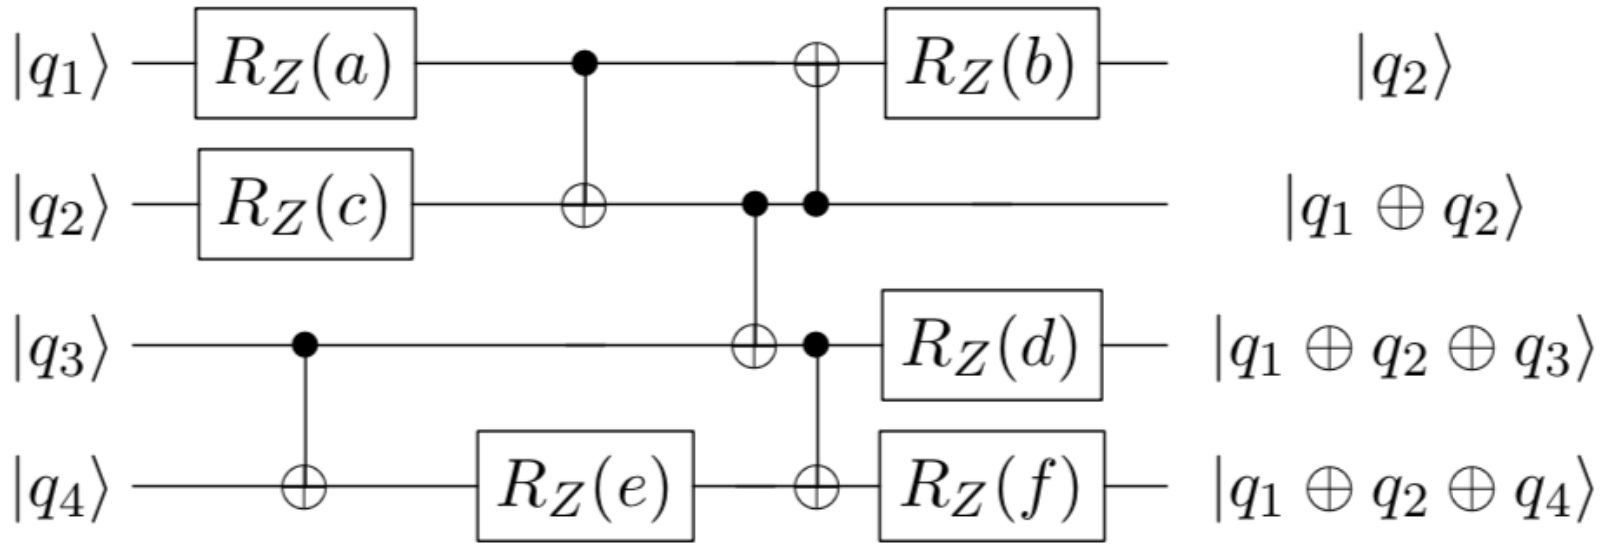
\includegraphics[width=.8\linewidth]{figure/parity.png}
        \caption{CNOT + phase circuit example}
    \end{figure}
\end{frame}
\subsection{CNOT + phase circuit + hadamard}
\begin{frame}
    \frametitle{universal set}
    \begin{itemize}
        \item $\left\{CNOT,S,T,S^{\dagger},T^{\dagger},H\right\}$
        \item for a circuit $C$, $S_{k, CNOT} S_{k, H} \ldots S_{1, CNOT} S_{1, H}=C$
    \end{itemize}
\end{frame}
\subsection{result}
\begin{frame}
    \frametitle{results for CNOT + $R_Z$}
    \begin{figure}
        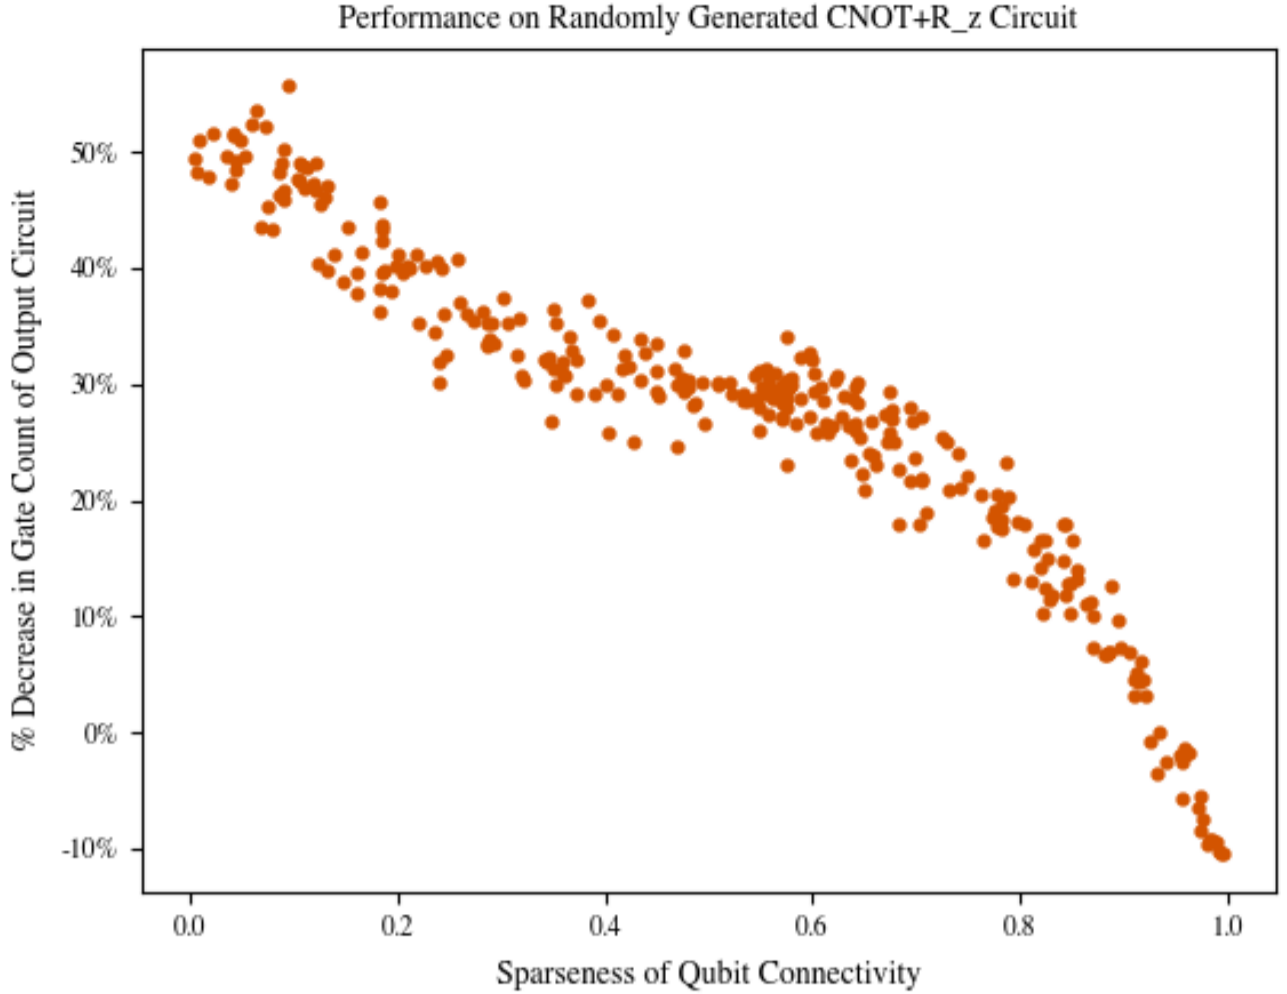
\includegraphics[width=.6\linewidth]{figure/CNOT+Rz.png}
        \caption{results for the synthesis of $CNOT + R_Z$ circuits on 20 qubits}
    \end{figure}
\end{frame}
\begin{frame}
    \frametitle{results for universal sets}
    \begin{figure}
        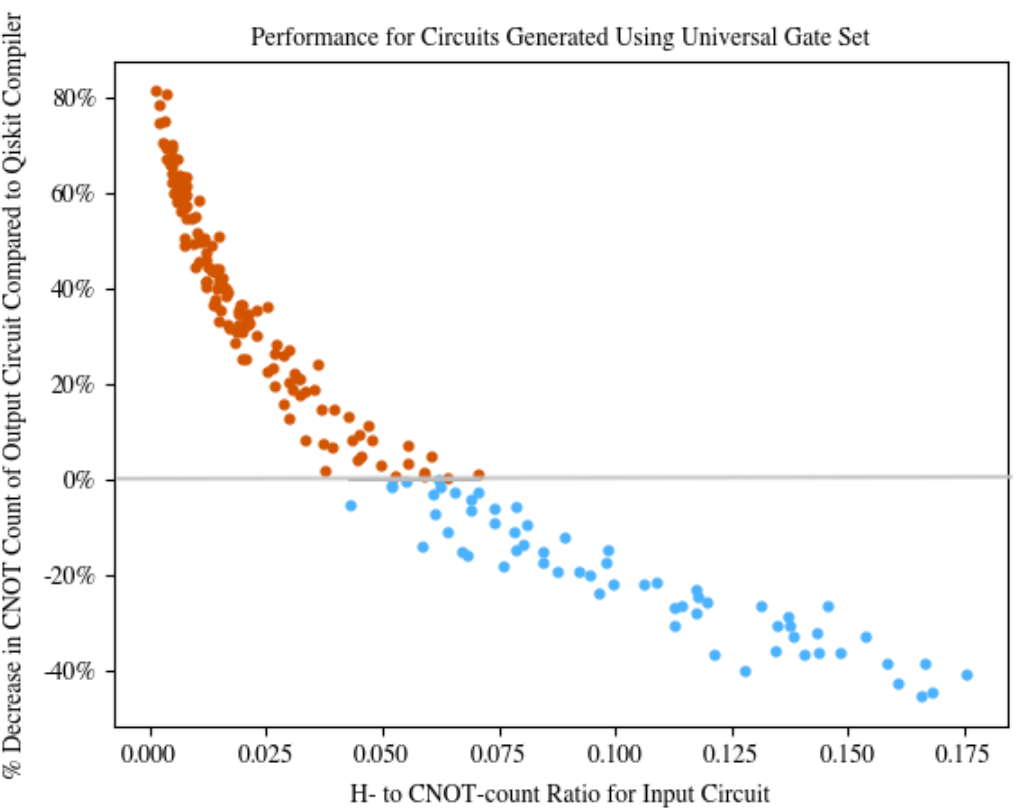
\includegraphics[width=.6\linewidth]{figure/universal.png}
        \caption{generate circuits from universal set $\left\{CNOT,S,T,S^{\dagger},T^{\dagger},H\right\}$ compared with IBM's compiler}
    \end{figure}
\end{frame}